%%%%%%%%%%%%%%%%%%%%%%%%%%%%%%%%%%%%%%%%%
% Masters/Doctoral Thesis 
% LaTeX Template
% Version 2.5 (27/8/17)
%
% This template was downloaded from:
% http://www.LaTeXTemplates.com
%
% Version 2.x major modifications by:
% Vel (vel@latextemplates.com)
%
% This template is based on a template by:
% Steve Gunn (http://users.ecs.soton.ac.uk/srg/softwaretools/document/templates/)
% Sunil Patel (http://www.sunilpatel.co.uk/thesis-template/)
%
% Template license:
% CC BY-NC-SA 3.0 (http://creativecommons.org/licenses/by-nc-sa/3.0/)
%
%%%%%%%%%%%%%%%%%%%%%%%%%%%%%%%%%%%%%%%%%

%----------------------------------------------------------------------------------------
%  PACKAGES AND OTHER DOCUMENT CONFIGURATIONS
%----------------------------------------------------------------------------------------

\documentclass[
11pt, % The default document font size, options: 10pt, 11pt, 12pt
%oneside, % Two side (alternating margins) for binding by default, uncomment to switch to one side
english, % ngerman for German
singlespacing, % Single line spacing, alternatives: onehalfspacing or doublespacing
%draft, % Uncomment to enable draft mode (no pictures, no links, overfull hboxes indicated)
%nolistspacing, % If the document is onehalfspacing or doublespacing, uncomment this to set spacing in lists to single
%liststotoc, % Uncomment to add the list of figures/tables/etc to the table of contents
%toctotoc, % Uncomment to add the main table of contents to the table of contents
%parskip, % Uncomment to add space between paragraphs
%nohyperref, % Uncomment to not load the hyperref package
headsepline, % Uncomment to get a line under the header
%chapterinoneline, % Uncomment to place the chapter title next to the number on one line
%consistentlayout, % Uncomment to change the layout of the declaration, abstract and acknowledgements pages to match the default layout
]{MastersDoctoralThesis} % The class file specifying the document structure

\usepackage[utf8]{inputenc} % Required for inputting international characters
\usepackage[T1]{fontenc} % Output font encoding for international characters

\usepackage{mathpazo} % Use the Palatino font by default

\usepackage[backend=biber,style=authoryear,natbib=true]{biblatex}

\addbibresource{Bibliography.bib} % The filename of the bibliography

\usepackage[autostyle=true]{csquotes} % Required to generate language-dependent quotes in the bibliography

%----------------------------------------------------------------------------------------
%  EXTRA CONFIGURATIONS
%----------------------------------------------------------------------------------------



%----------------------------------------------------------------------------------------
%  MARGIN SETTINGS
%----------------------------------------------------------------------------------------

\geometry{
  paper=a4paper, % Change to letterpaper for US letter
  inner=2.5cm, % Inner margin
  outer=3.8cm, % Outer margin
  bindingoffset=.5cm, % Binding offset
  top=1.5cm, % Top margin
  bottom=1.5cm, % Bottom margin
  %showframe, % Uncomment to show how the type block is set on the page
}

%----------------------------------------------------------------------------------------
%  THESIS INFORMATION
%----------------------------------------------------------------------------------------

\thesistitle{Thesis Title} % Your thesis title, this is used in the title and abstract, print it elsewhere with \ttitle
\supervisor{Dr. James \textsc{Smith}} % Your supervisor's name, this is used in the title page, print it elsewhere with \supname
\examiner{} % Your examiner's name, this is not currently used anywhere in the template, print it elsewhere with \examname
\degree{Doctor of Philosophy} % Your degree name, this is used in the title page and abstract, print it elsewhere with \degreename
\author{John \textsc{Smith}} % Your name, this is used in the title page and abstract, print it elsewhere with \authorname
\addresses{} % Your address, this is not currently used anywhere in the template, print it elsewhere with \addressname

\subject{Biological Sciences} % Your subject area, this is not currently used anywhere in the template, print it elsewhere with \subjectname
\keywords{} % Keywords for your thesis, this is not currently used anywhere in the template, print it elsewhere with \keywordnames
\university{\href{http://www.university.com}{University Name}} % Your university's name and URL, this is used in the title page and abstract, print it elsewhere with \univname
\department{\href{http://department.university.com}{Department or School Name}} % Your department's name and URL, this is used in the title page and abstract, print it elsewhere with \deptname
\group{\href{http://researchgroup.university.com}{Research Group Name}} % Your research group's name and URL, this is used in the title page, print it elsewhere with \groupname
\faculty{\href{http://faculty.university.com}{Faculty Name}} % Your faculty's name and URL, this is used in the title page and abstract, print it elsewhere with \facname

\AtBeginDocument{
\hypersetup{pdftitle=\ttitle} % Set the PDF's title to your title
\hypersetup{pdfauthor=\authorname} % Set the PDF's author to your name
\hypersetup{pdfkeywords=\keywordnames} % Set the PDF's keywords to your keywords
}

\begin{document}

\frontmatter % Use roman page numbering style (i, ii, iii, iv...) for the pre-content pages

\pagestyle{plain} % Default to the plain heading style until the thesis style is called for the body content

%----------------------------------------------------------------------------------------
%  TITLE PAGE
%----------------------------------------------------------------------------------------

\begin{titlepage}
\begin{center}

\vspace*{.06\textheight}
{\scshape\LARGE \univname\par}\vspace{1.5cm} % University name
\textsc{\Large Doctoral Thesis}\\[0.5cm] % Thesis type

\HRule \\[0.4cm] % Horizontal line
{\huge \bfseries \ttitle\par}\vspace{0.4cm} % Thesis title
\HRule \\[1.5cm] % Horizontal line
 
\begin{minipage}[t]{0.4\textwidth}
\begin{flushleft} \large
\emph{Author:}\\
\href{http://www.johnsmith.com}{\authorname} % Author name - remove the \href bracket to remove the link
\end{flushleft}
\end{minipage}
\begin{minipage}[t]{0.4\textwidth}
\begin{flushright} \large
\emph{Supervisor:} \\
\href{http://www.jamessmith.com}{\supname} % Supervisor name - remove the \href bracket to remove the link  
\end{flushright}
\end{minipage}\\[3cm]
 
\vfill

\large \textit{A thesis submitted in fulfillment of the requirements\\ for the degree of \degreename}\\[0.3cm] % University requirement text
\textit{in the}\\[0.4cm]
\groupname\\\deptname\\[2cm] % Research group name and department name
 
\vfill

{\large \today}\\[4cm] % Date
%\includegraphics{Logo} % University/department logo - uncomment to place it
 
\vfill
\end{center}
\end{titlepage}

%----------------------------------------------------------------------------------------
%  DECLARATION PAGE
%----------------------------------------------------------------------------------------

\begin{declaration}
\addchaptertocentry{\authorshipname} % Add the declaration to the table of contents
\noindent I, \authorname, declare that this thesis titled, \enquote{\ttitle} and the work presented in it are my own. I confirm that:

\begin{itemize} 
\item This work was done wholly or mainly while in candidature for a research degree at this University.
\item Where any part of this thesis has previously been submitted for a degree or any other qualification at this University or any other institution, this has been clearly stated.
\item Where I have consulted the published work of others, this is always clearly attributed.
\item Where I have quoted from the work of others, the source is always given. With the exception of such quotations, this thesis is entirely my own work.
\item I have acknowledged all main sources of help.
\item Where the thesis is based on work done by myself jointly with others, I have made clear exactly what was done by others and what I have contributed myself.\\
\end{itemize}
 
\noindent Signed:\\
\rule[0.5em]{25em}{0.5pt} % This prints a line for the signature
 
\noindent Date:\\
\rule[0.5em]{25em}{0.5pt} % This prints a line to write the date
\end{declaration}

\cleardoublepage

%----------------------------------------------------------------------------------------
%  ABSTRACT PAGE
%----------------------------------------------------------------------------------------

\begin{abstract}
\addchaptertocentry{\abstractname} % Add the abstract to the table of contents
The Thesis Abstract is written here (and usually kept to just this page). The page is kept centered vertically so can expand into the blank space above the title too\ldots
\end{abstract}

%----------------------------------------------------------------------------------------
%  ACKNOWLEDGEMENTS
%----------------------------------------------------------------------------------------

\begin{acknowledgements}
\addchaptertocentry{\acknowledgementname} % Add the acknowledgements to the table of contents
The acknowledgments and the people to thank go here, don't forget to include your project advisor\ldots
\end{acknowledgements}

%----------------------------------------------------------------------------------------
%  TABLE OF CONTENTS
%----------------------------------------------------------------------------------------

\tableofcontents

%----------------------------------------------------------------------------------------
%  ABBREVIATIONS
%----------------------------------------------------------------------------------------

\begin{abbreviations}{ll} % Include a list of abbreviations (a table of two columns)

\textbf{LAH} & \textbf{L}ist \textbf{A}bbreviations \textbf{H}ere\\
\textbf{WSF} & \textbf{W}hat (it) \textbf{S}tands \textbf{F}or\\

\end{abbreviations}

%----------------------------------------------------------------------------------------
%  PHYSICAL CONSTANTS/OTHER DEFINITIONS
%----------------------------------------------------------------------------------------

\begin{constants}{lr@{${}={}$}l} % The list of physical constants is a three column table

% The \SI{}{} command is provided by the siunitx package, see its documentation for instructions on how to use it

Speed of Light & $c_{0}$ & \SI{2.99792458e8}{\meter\per\second} (exact)\\
%Constant Name & $Symbol$ & $Constant Value$ with units\\

\end{constants}

%----------------------------------------------------------------------------------------
%  SYMBOLS
%----------------------------------------------------------------------------------------

\begin{symbols}{lll} % Include a list of Symbols (a three column table)

$a$ & distance & \si{\meter} \\
$P$ & power & \si{\watt} (\si{\joule\per\second}) \\
%Symbol & Name & Unit \\

\addlinespace % Gap to separate the Roman symbols from the Greek

$\omega$ & angular frequency & \si{\radian} \\

\end{symbols}

%----------------------------------------------------------------------------------------
%  THESIS BODY
%----------------------------------------------------------------------------------------

\mainmatter % Begin numeric (1,2,3...) page numbering

\pagestyle{thesis} % Return the page headers back to the "thesis" style

% Include the chapters of the thesis as separate files from the Chapters folder
% Uncomment the lines as you write the chapters

\chapter{Introduction}
\label{chp:introduction}
%----------------------------------------------------------------------------------------

% Define some commands to keep the formatting separated from the content 
\newcommand{\keyword}[1]{\textbf{#1}}
\newcommand{\tabhead}[1]{\textbf{#1}}
\newcommand{\code}[1]{\texttt{#1}}
\newcommand{\file}[1]{\texttt{\bfseries#1}}
\newcommand{\option}[1]{\texttt{\itshape#1}}

%----------------------------------------------------------------------------------------



Flooding and inundation have dramatically increased in the last years due to climate change.
The frequency, as well as the magnitude of extreme rain events, leading to major inundations, have grown, making our capability to predict occurrence and effects more unreliable.
To limit risks and damage, novel control, mitigation and warning measures are needed.
Design and implementation of these need preliminary study of the situation based on data and information.
Unfortunately, these are often not available, or not in the amount required for carrying out preliminary studies.

Nowadays simulation offers a valid and very powerful tool for dealing with this problem.
Hydrological numerical models of catchments can be built, where depending on the degree of detail required different processes are implemented: infiltration, evaporation, erosion, etc.
Depending on the degree of detail chosen more or less accurate models can be achieved.
These models are mainly based on topographical data of the catchment in question, which are then refined by assigning friction coefficients values, infiltration capacity values, hydraulic conductivity values, porosity values to the different zones of the catchment.
Such models need to be calibrated.
This means that by using optimization algorithms the parameters of the model are varied within certain ranges in order to reproduce at best a recorded output (e.g. river outlet hydrograph) generated from "known" initial conditions (e.g. initial soil saturation) and inputs (e.g. the recorded hyetograph).
Once the model is calibrated it can be used to generate new data, from which new information about the given system can be learned and from which other conditions and new situations can be tested.

The main drawback of simulation lays in its very high computational burden.
For calibration alone several runs of the model are required.
Every simulation can last from some minutes up to several hours, depending on the complexity of the model, the type of computer where the simulations are run, the duration of the event simulated, the resolution used for the model, etc.
Once the model is calibrated several more runs are necessary in order to generate the desired dataset.
The number of runs depends on the kind of study one would like to carry out.
For uncertainty analysis for example, up to some thousands of simulations can be run, in order to study the influence that the variation of a parameter of the model (or its uncertain determination) has on the output.\\

\ldots\\



\seb{Rearrange and somehow integrate the two previous sections in order to produce a global introduction. Introduce the following section "Emulation", a brief introduction about emulation}

% ---------------------------------------------------------------------------------------------------
% ===================================================================================================
\section{Definition of goals}
% ===================================================================================================

Focus on emulation subject.

\begin{itemize}
\itemsep0em
  \item explain what is emulation
  \item use both terms \textit{surrogate model} and \textit{emulator}
  \item mention \textit{EmuMore} project
  \item give emulation examples
\end{itemize}


% ==============================================================================
\section{Emulation}
% ==============================================================================

\begin{itemize}
\itemsep0em
  \item define the goals of this thesis
  \item state the questions which should be answered withing this thesis. Try to close the loop in the conclusions chapter (cf. Thesis example Jörg)
  \item what readers should expect from the thesis
  \item mention reproducibility, open softwares
  \item include a scheme with the \emph{emulation workflow}
\end{itemize}









\chapter{Related work}
\label{chp:related_work}

\section{Regression and interpolation}

\section{Development GNU Octave package \textit{fswof2d}}

\section{Mechanistic emulator weir equation}

\chapter{Early flood warning tool}
\label{chp:flood_warning_system}

An \textit{early flood warning tool} in an essential component of an \textit{early flood warning system}.
An early flood warning system has to be understood as an integrated system of tools and plans to detect and respond to flood emergencies \autocite{icimod_early_2018}.
This can be managed by the community themselves and if designed, implemented and operated correctly can make the difference between tragedy and survival.

Such systems have already been installed in various endangered regions in the world.
After the major flooding of July 2014, the city of Altstätten in the canton of St. Gallen made the decision to install one.
The system installed uses cameras, sensors and level meters to gather data and information about the current situation \autocite{st._galler_tageblatt_altstatten_2017}.
When the value of certain parameters exceed the given threshold, a dangerous situation is recognized and the alarm signal is sent.

Three years after the installation of the system an alarm rings in the middle of the night.
Firemen go immediately into action in order to install temporary measures to fight against the water.
A couple of hours later the torrent overflows at several points and the city gets flooded.
Damages are less severe than last time, especially thanks to the temporary measures installed, but possibly they could have been reduced even more.

Crucial in order to limit the damages is the intervention time before the actual flooding occurs.
The earlier the dangerous situation can be detected the more time is available to the population and authorities to get ready and set up different types of temporary mitigation measures.
Systems based on sensors monitoring the evolution of the current situation in the upper part of the catchment are quite reliable but do not allow for long anticipation time. 

Numerical simulations can be run with meteorological forcast data and approximate soil saturation conditions in order to obtain early predictions of the event outcome.
However, the big advantage of predicting with that much anticipation is partially lost due to the duration of such simulations.
Accurate meteorological forcasts are available only few hours before the event.
If the model require several hours to run, which is often the case to obtain accurate predictions for catchments of this extent, then the advantage of being able to run it in advance is cancelled.

A possible solution to this problem is the developement of an \emph{ad hoc surrogate model} exploiting the catchment specific behaviour.


\section{Methodology}

In order to run the simulations necessary for building the emulator, a synthetic topography was produced.
The synthetic topography, in comparison with a real one, 

Bla bla bla bla \autocite{octave_community_gnu_2018}.

\begin{figure}[htpb]
  \centering
  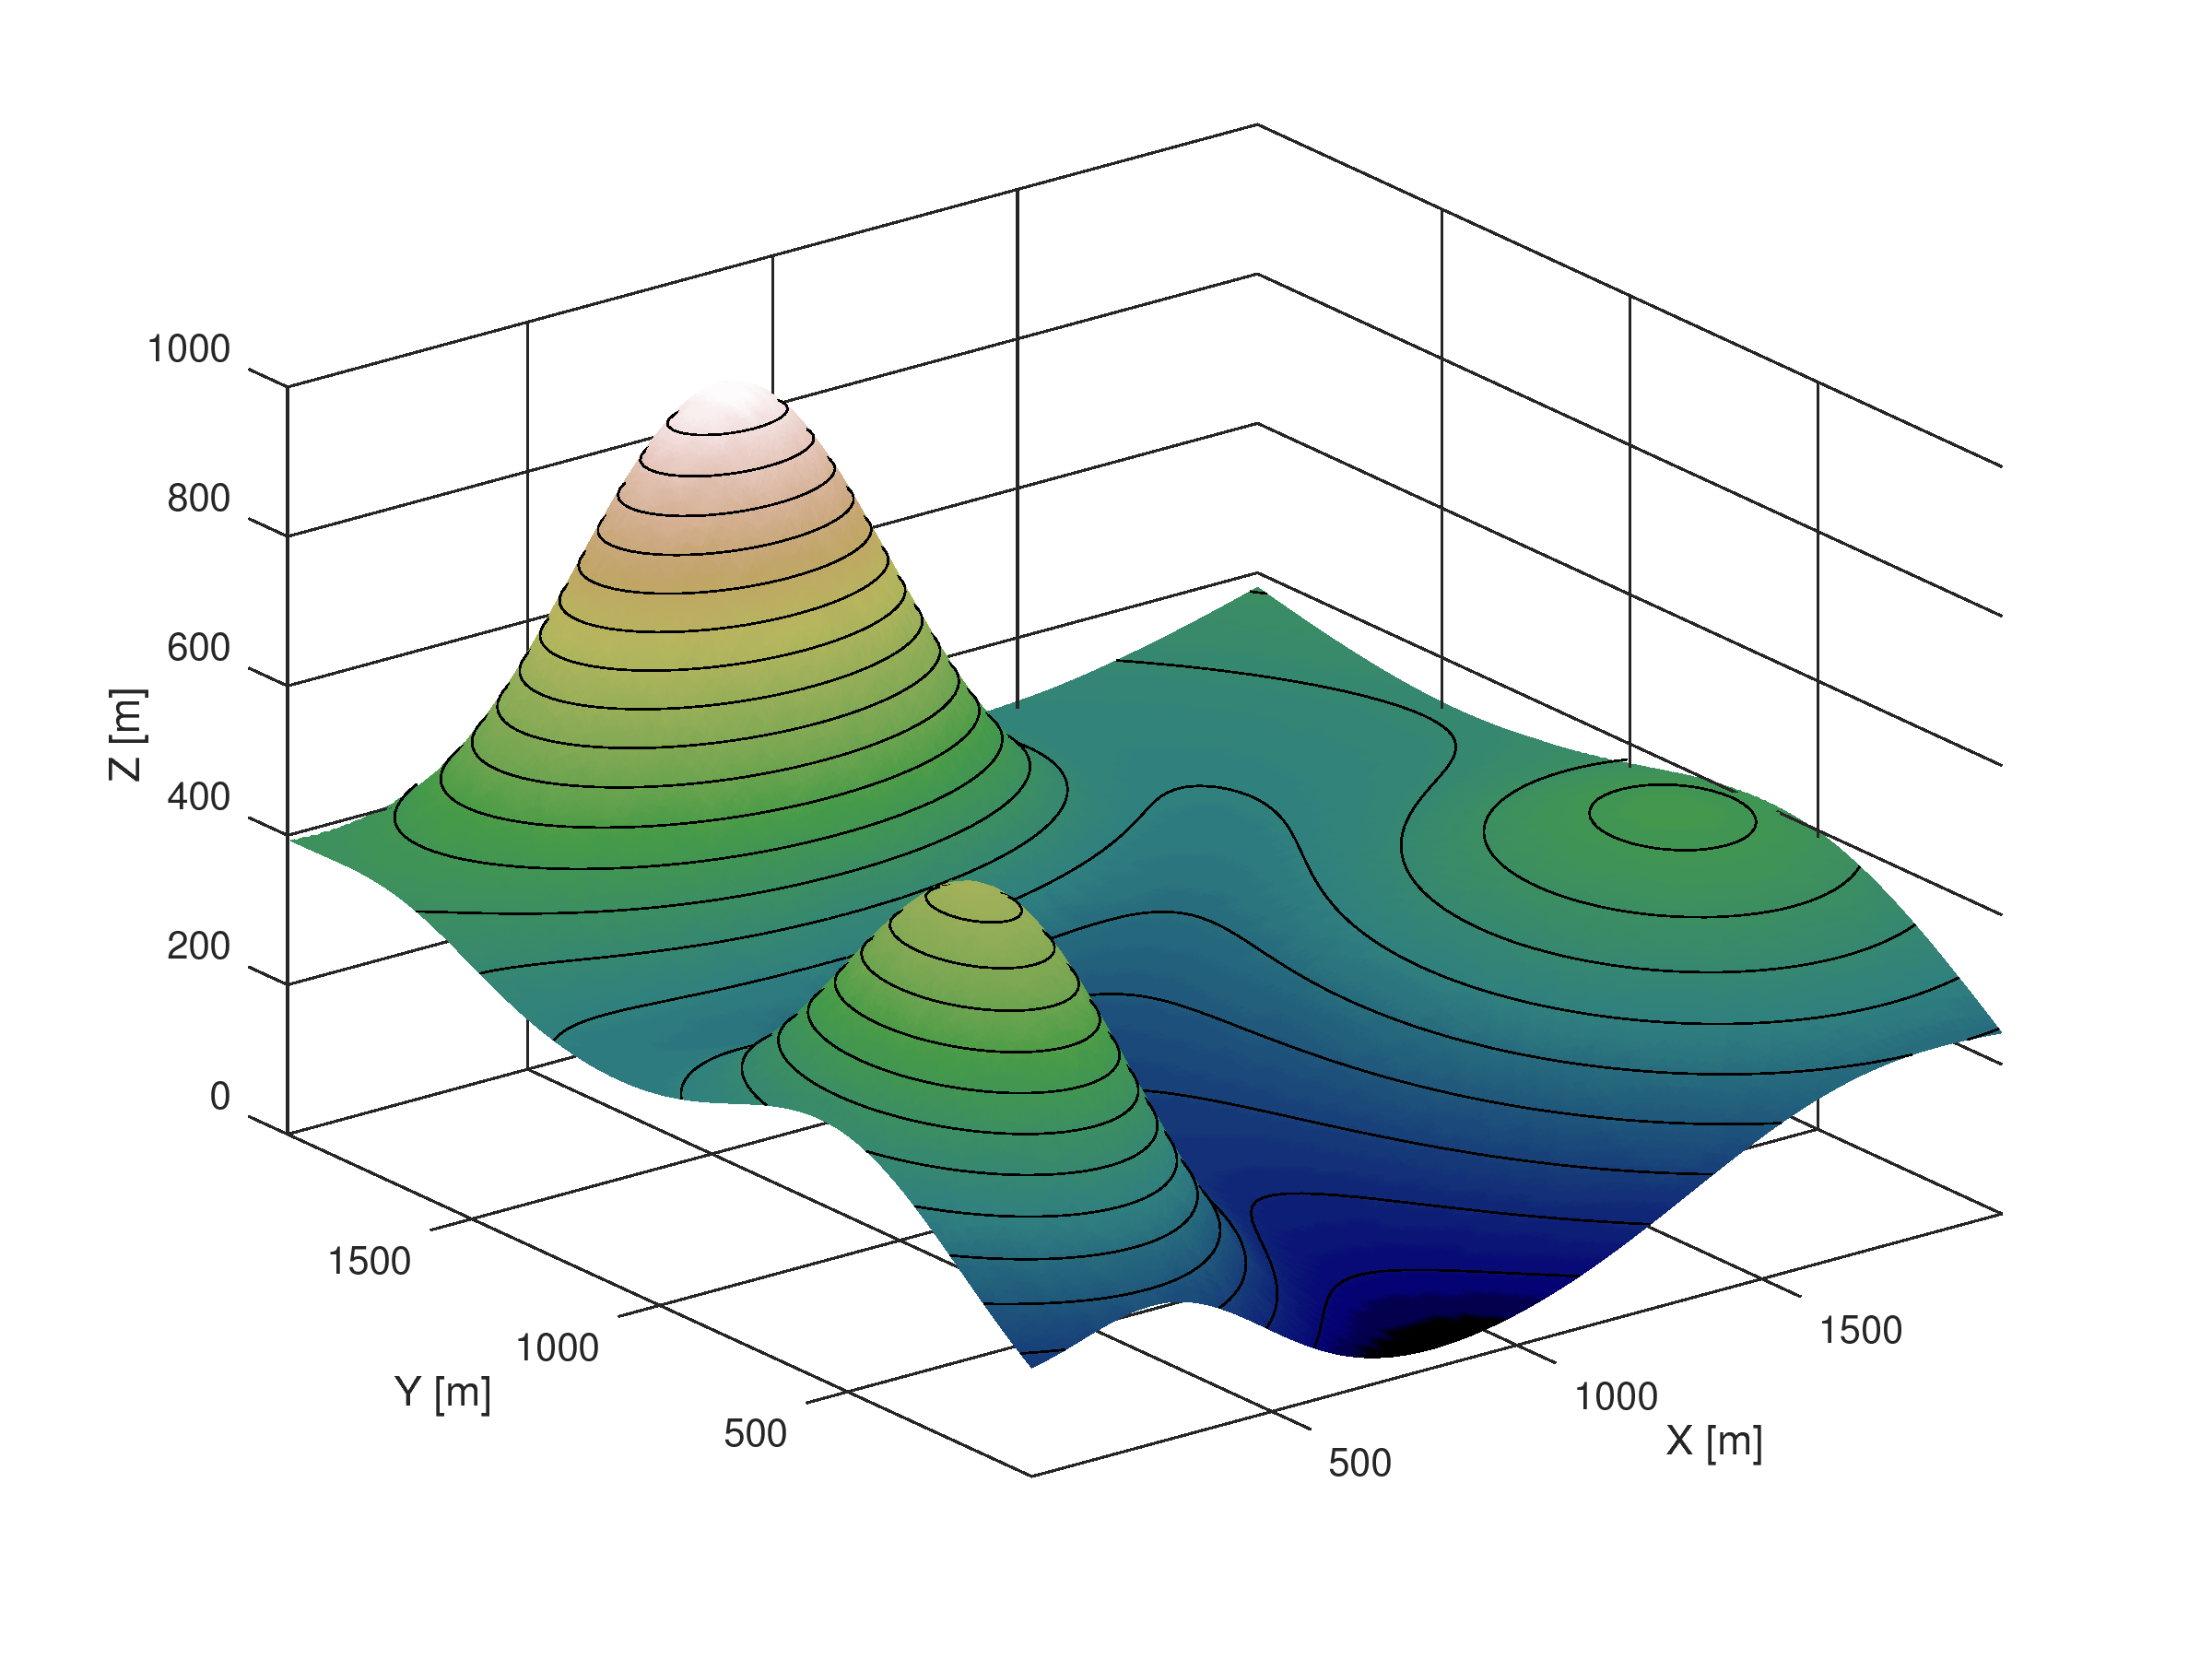
\includegraphics[width=0.7\textwidth]{../../../img/topography.png}
  \caption{Synthetic topography composed of three gaussian bumps on a sloping plane. A parabola centered on the middle axis of the plane was added to favour concentration of the flow towards the center.}
  \label{fig:topography}
\end{figure}

\section{Results}


\chapter{Discussion}
\label{chp:conclusions}



\chapter{Conclusions}
\label{chp:outlook}




%individual results are probably being discussed in 3.1.2 and 3.2.2

%Here, you could provide a joint discussion, maybe discussion common features/insight for both case studies. FullSwof, GPs as tools vs. "simple" emulators such as response surfaces/lin. methods.

%Also, you could move the next steps/outlook part here.



%probably move bullet points 2 and 3 to discussion section and have Conclusion as summarizing section, re-stating the problem, the general approach, the main results (Answers to Research questions). and brief summary of future work.


%5.1. Answers to research questions

%5.2. Open questions


%s of this thesis.

%You can stay with "Goals", or break it down into different "objectives"/sub-goals, if needed.

%From goals/objectives, usually research questions are derived. These should be as specific as possible, so you can write a concise answer.





%The work done on emulation 

This thesis follows a storyline, which connects up the dots, resulting in a prelude to emulation for near-time flood prediction.
Venturing in a completely new field, that of emulation, opened me up a whole new world.
This itinerary through emulation, after clearing up some initial doubts, made me realize its true potential.
Emulation can have great applicability, especially in the engineering fields.
Engineering often has to tackle repetitive problems, which solution can be found only iteratively.
Emulation can provide alternative new ways to solve such problems.
Once an appropriate emulator for a specific task is built, this can provide fast answer to the problem of interest.
Emulation can be performed at almost no cost: it requires neither special tools nor special investments.
The work done on this thesis demonstrate it.\\

In spite of its simplicity, the first case study was for me a very didactic one.
The weir equation, commonly used in hydraulic engineering, proved to be a fair approximation of the relation discharge-height over the weir, although flexible non parametric interpolation techniques have shown to produce more accurate estimates when an adequate number of observations is available.
This case study also shows the potential of numerical simulation in replacing the realization of laboratory experiments, with the potential of reducing future research costs and time.\\

Although the methodology in the second case study appears more complex than the one adopted in the first one, the high level of abstraction and generalization of the presented workflow allows to apply the proposed early flood warning system to real situations with only slight modifications. These especially concerns the assessment of the emulator performance. Still, the partial accuracy assessment conducted reported excellent performance, especially with regards to the estimation of the time period before a flood occurs. \\

In conclusion, this thesis shows the benefit of conjugating the accuracy of numerical simulation with the huge enhancement in computing time provided by emulators. In the engineering field, promising research areas may include uncertainty propagation, sensitivity analysis and models optimization or calibration, which are actually hampered by the excessive computational burden of numerical simulation. 


 
% - automatization
% - to bridge a gap
% innovation

 
 

 




















%----------------------------------------------------------------------------------------
%  BIBLIOGRAPHY
%----------------------------------------------------------------------------------------

\printbibliography[heading=bibintoc]

%----------------------------------------------------------------------------------------
%  APPENDIX
%----------------------------------------------------------------------------------------

\appendix % Cue to tell LaTeX that the following "chapters" are Appendices

% Include the appendices of the thesis as separate files from the Appendices folder
% Uncomment the lines as you write the Appendices

% Appendix A

\chapter{Frequently Asked Questions} % Main appendix title

\label{AppendixA} % For referencing this appendix elsewhere, use \ref{AppendixA}

\section{How do I change the colors of links?}

The color of links can be changed to your liking using:

{\small\verb!\hypersetup{urlcolor=red}!}, or

{\small\verb!\hypersetup{citecolor=green}!}, or

{\small\verb!\hypersetup{allcolor=blue}!}.

\noindent If you want to completely hide the links, you can use:

{\small\verb!\hypersetup{allcolors=.}!}, or even better: 

{\small\verb!\hypersetup{hidelinks}!}.

\noindent If you want to have obvious links in the PDF but not the printed text, use:

{\small\verb!\hypersetup{colorlinks=false}!}.


%----------------------------------------------------------------------------------------

\end{document}  
